\documentclass[3p, authoryear]{elsarticle} %review=doublespace preprint=single 5p=2 column
%%% Begin My package additions %%%%%%%%%%%%%%%%%%%
\usepackage[hyphens]{url}

  \journal{Submitted to NARSC 2021} % Sets Journal name


\usepackage{lineno} % add
\providecommand{\tightlist}{%
  \setlength{\itemsep}{0pt}\setlength{\parskip}{0pt}}

\usepackage{graphicx}
\usepackage{booktabs} % book-quality tables
%%%%%%%%%%%%%%%% end my additions to header

\usepackage[T1]{fontenc}
\usepackage{lmodern}
\usepackage{amssymb,amsmath}
\usepackage{ifxetex,ifluatex}
\usepackage{fixltx2e} % provides \textsubscript
% use upquote if available, for straight quotes in verbatim environments
\IfFileExists{upquote.sty}{\usepackage{upquote}}{}
\ifnum 0\ifxetex 1\fi\ifluatex 1\fi=0 % if pdftex
  \usepackage[utf8]{inputenc}
\else % if luatex or xelatex
  \usepackage{fontspec}
  \ifxetex
    \usepackage{xltxtra,xunicode}
  \fi
  \defaultfontfeatures{Mapping=tex-text,Scale=MatchLowercase}
  \newcommand{\euro}{€}
\fi
% use microtype if available
\IfFileExists{microtype.sty}{\usepackage{microtype}}{}
\usepackage{natbib}
\bibliographystyle{apalike}
\usepackage{longtable}
\usepackage{graphicx}
\ifxetex
  \usepackage[setpagesize=false, % page size defined by xetex
              unicode=false, % unicode breaks when used with xetex
              xetex]{hyperref}
\else
  \usepackage[unicode=true]{hyperref}
\fi
\hypersetup{breaklinks=true,
            bookmarks=true,
            pdfauthor={},
            pdftitle={Utility-Based Accessibility to Community Resources: An Application of Location-Based Services Data},
            colorlinks=false,
            urlcolor=blue,
            linkcolor=magenta,
            pdfborder={0 0 0}}
\urlstyle{same}  % don't use monospace font for urls

\setcounter{secnumdepth}{5}
% Pandoc toggle for numbering sections (defaults to be off)

% Pandoc citation processing

% Pandoc header
\usepackage{booktabs}
\usepackage{booktabs}
\usepackage{longtable}
\usepackage{array}
\usepackage{multirow}
\usepackage{wrapfig}
\usepackage{float}
\usepackage{colortbl}
\usepackage{pdflscape}
\usepackage{tabu}
\usepackage{threeparttable}
\usepackage{threeparttablex}
\usepackage[normalem]{ulem}
\usepackage{makecell}
\usepackage{xcolor}



\begin{document}
\begin{frontmatter}

  \title{Utility-Based Accessibility to Community Resources: An Application of Location-Based Services Data}
    \author[BYU]{Gregory Macfarlane\corref{1}}
   \ead{gregmacfarlane@byu.edu} 
    \author[BYU]{Emma Stucki}
   \ead{stuckiemma@gmail.com} 
    \author[BYU]{Michael Copley}
  
    \author[]{}
  
        \cortext[1]{Corresponding Author}
  
  \begin{abstract}
  Understanding who in a community has access to its resources -- parks, libraries, grocery stores, etc. -- has profound equity implications, but typical methods to understand access to these resources are limited. Travel time buffers require researchers to assert mode of access as well as an arbitrary distance threshold; further, these methods do not distinguish between destination quality attributes in an effective way. In this research, we present a methodology to develop utility-based accessibility measures for parks, libraries, and grocery stores in Utah County, Utah. The method relies on passive location-based services data to model destination choice to these community resources; the destination choice model utility functions in turn allow us to develop a picture of regional access that is sensitive to: the quality and size of the destination resource; continuous (non-binary) travel impedance by multiple modes; and the sociodemographic attributes of the traveler. We then use this measure to explore equity in access to the specified community resources across income level and minority status in Utah County.
  \end{abstract}
   \begin{keyword} Accessibility Passive Data Location Choice\end{keyword}
 \end{frontmatter}

\hypertarget{intro}{%
\section{Introduction}\label{intro}}

Communities provide important resources to their members, and spatial exclusion
from these resources can negatively affect both subjective measures of well-being
\citep{currie2010modeling} and economic opportunity.
Measuring good or poor access to these resources is an important concern. But
access involves more than merely distance or travel impedance: it is a function
of the quality of the resource, and how many options for the resource are
available.

In this paper, we consider utility-based access to parks, grocery stores, and
libraries in Utah County, Utah. The utility preferences are estimated on
location-based services data obtained from a third-party commercial data
aggregator. We then use the model estimates to construct a composite
accessibility measure and compare the measure with neighborhood-level
sociodemographic characteristics.

The paper begins with a discussion of previous attempts to evaluate
access to community resources. We then describe the methodology employed in
this research, which makes use of novel third-party datasets

\hypertarget{lit-review}{%
\section{Literature}\label{lit-review}}

Research about accessibility in the recent years has placed a considerable focus
on access to jobs and the corresponding negative impact that there is on a
community when there is a lack of accessibility to quality jobs. A research
study was done examining job accessibility of the poor in Los Angeles to
determine whether it was a problem in accessibility that caused the employment
distribution pattern that is present in the cities today. This research was done
to address an issue that is caused by not having access to jobs, and they found
similar results to much of the other research that has been done, in that there
are jobs that are accessible in the poor city centers, but the number of jobs is
declining. So although there is access, the lack of access is concerning when
considering the impact it could have on communities that are already struggling
(Hu, 2015). In a similar research study done in Australia that examined
accessibility to jobs, they connected accessibility of jobs to sense of
well-being and satisfaction with life. In this study they found that transport
disadvantage is positively associated with social exclusion (where their
definition of social exclusion means comparatively less access to employment,
shops, and other entertainment) and social exclusion is strongly negatively
associated with well-being, showing an overall conclusion that social exclusion
contributes to poor well being and transport disadvantage contributes to social
exclusion \citep{currie2010modeling}. Both of these research studies showed the
effect of lack of access to jobs, but neither really discussed the effects of
limited accessibility to other public resources such as parks and greenspace,
grocery stores, and libraries.

There is comparatively little research that has been done on the subject, but
one article does specifically address nonwork accessibility and its impact on
vulnerable social groups. \citet{grengs2015nonwork} found that when looking at
accessibility among vulnerable social groups such as African Americans,
Hispanics, low-income households, and households in poverty, there is a
substantially larger share of households with extreme levels of low
accessibility and so they share a remarkable disadvantage in accessibility to
shopping and supermarkets. This research used a gravity model and included the
impedance factor from traveling between origin and destination as well as the
attractiveness factor based on the number of opportunities in the destination
zone. The model of accessibility is relatively robust in including
attractiveness and impedance for the different zones, however, the
attractiveness part of the equation was entirely based upon the number of
opportunities in the destination. Even this research lacks a study based upon
what amenity is most attractive to people for a particular resource, and whether
or not they have access to that amenity. For example, in a grocery store, is it
more desirable to have more fresh produce or lower prices? Then using that
information, does the person have access to the resources that they want? These
variables help us identify the potential reach accessibility needs to have for a
particular resource. In our study we will attempt to analyze different variables
that could contribute to the attractiveness of a resource for parks and
greenspace, grocery stores, and libraries.

We have chosen to analyze these resources because of several reasons, including
their popularity in the community, the availability of existing data to collect,
and the negative or positive impacts having access to these resources has on
physical and emotional well-being.

One of the resources that we are analyzing is libraries. They are a space that
allows people to gather to learn, escape pressures of life, connect with others,
and socialize in a way that is different than any other community building. In
addition, libraries are a community resource that are almost entirely supported
by the local community. (Kalikow Maxwell, 2008) Libraries are indoor spaces that
are free for public use, and available in most communities. In a major study of
residential environments, libraries were found to be more popular than any other
amenity except a food or drugstore. This was true for every demographic.
However, despite its popularity and social benefit, libraries are still not very
prevalent. According to the statistical abstract there are 39,400 pharmacies,
67,000 supermarkets and only 16,192 public libraries in the U.S. For the third
most desired community resource, the number of libraries is remarkably low, and
thus it is essential to improve accessibility to this resource. Additionally,
libraries provide a place to gather together and learn together with other
members of the community. Many stories of the aftermath of the tragedy of 9/11
tell how much of the community went to the library in search of information and
community feeling and to gather together in their loss. Because libraries are a
free resource, they are available to every demographic and something that is
important to all \citep{barclay2017space}

Parks fill a niche that is similar to libraries: just as libraries provide
places for community gatherings and self-improvement, so do parks. Some of the
reasons parks are essential are because of their benefit to mental health and
physical health. Parks and other greenspace have been the subject of research
when comparing access to parks and the influence on mental health. In a study
done on young adults and teens and their access to green space, it was found
that an increase in access to greenspace corresponded to a decrease in
likelihood of anxiety, depression, or another mental health disorder. (Madzia et
al., 2019) This research noted that some parks are more desirable than others
because of their environment or community. People may not feel safe in a certain
place and be less likely to frequent a park for that reason, and so may not
receive the benefits of the park close by. Yet there also may be other reasons
not to frequent a park, such as low upkeep, lack of shade, or lack of amenities
and play equipment for children or adults. One aspect that we will be analyzing
in this research is what qualities of parks are more desirable, such as more
vegetation, or trails, or sports courts, or playgrounds. All of these factors
contribute to what draws a person to a particular park and can help us identify
how to improve parks that are existing and not used as much because of a
previously unknown variable. In addition to improving mental health as was
analyzed in this research, parks can also provide ways to exercise and become
healthy. In a review done about the proximity and density of parks and physical
activity in the United States it was found that several studies found a positive
correlation between proximity to parks and physical activity, and in the studies
that compared multiple measurements and used smaller buffer sizes there was a
stronger correlation between parks and physical activity \citep{bancroft2015association}.
Although this is somewhat inconclusive, it is a factor that could be a positive
impact on health for those within access to parks.

The community resource that has many proven studies that show a correlation
between health and accessibility are grocery stores. Research that has been done
on this subject has termed lack of accessibility to fresh produce in grocery
stores as `food deserts'. These food deserts are often located in areas with a
low-income demographic, or a high percentage of minority population. As a
result, these groups have less access to healthy foods and are more likely to
have negative health effects. In a study done comparing access to supermarkets
and fruit and vegetable consumption, it was found that when only looking at
distance to nearest grocery store there was not a significant correlation
between shopping and fruit and vegetable consumption. However, this study also
found that many people passed their nearest option to go to a different
supermarket for their primary shopping, and those who shopped at less expensive
grocery stores had a corresponding diet with fewer fruits and vegetables \citep{aggarwal2014access}.
Therefore, in addition to access to healthy foods, it is
also personal choice that perhaps causes those in lower economic classes to
choose to forgo healthier options for cheaper options. These lower income
demographics also frequently do not have easy access to locations that accept
food stamps, or other places, such as food pantries, where they can get access
to healthier food options at an affordable price for their income. In a study
done on access to fresh produce in low-income neighborhoods in Los Angeles it
was found that only 41\% of food pantry clients were within walking distance of
stores with fresh produce, 83\% were within walking distance of stores with
limited produce, and 13\% were not within walking distance of either store type.
(Algert et al., 2006) Grocery store accessibility is important for other
demographic groups as well for the same reasons, and despite the seemingly
common presence of grocery stores throughout a city, we can see from this study
there are still locations and people that experience a lack of accessibility.

Because of the benefit of having these resources close, it is important to
identify what exactly makes something accessible. There are many different ways
of defining accessibility including isochrone, distance, community-based, and
network based. The isochrone definition of accessibility is defined as being
based on location, such as whether or not you are within a mile of a certain
resource. Algert et al.~used this basis for their accessibility model when
determining accessibility of low-income neighborhoods to healthy foods in Los
Angeles. They used a network distance model, tracing roads a distance of 0.8 km.
in every direction originating from each store location. (Algert et al., 2006)
This idea of accessibility is limited because it fails to include different
modes of travel or routes to go to the grocery store, such as on the way back
from work. In addition, it also fails to include time accessibility as well as
different variables such as familiarity, price comparison, or availability of
food groups, that may encourage or dissuade a person from visiting a particular
store.
Another accessibility measure is the distance model, which determines
accessibility by how close the nearest amenity is to a certain location. This
definition of accessibility is slightly more variable than the isochrone method
because it includes multiple stores in the method and includes stores that are
perhaps a little further away but could be reached using different modes of
transportation. But like the isochrone method, this does not use individual
level measures such as activity patterns or personal preferences. This method
was used in research done by Clifton to determine food availability for
low-income families in Texas. This study was able to determine and use different
mobility strategies, such as auto, rides, transit, walking, borrowing, taxis,
etc. They also included an additional variable that questioned the distance to
preferred supermarkets over distance to nearest supermarkets.(Clifton, 2004)
This variable adds an individual level to the model in addition to the simple
distance model. However, it still lacked the whole individual space time
environment and included just a few distinct variables.

The community-based model of accessibility is probably one of the most
simplistic definitions of accessibility of these four. This model is primarily
used to determine if a particular resource is located in a particular city or
county. This model could be helpful for resources that are perhaps not quite as
prevalent such as hospitals or libraries, or for relatively small cities.
However, for resources that are more common like parks and grocery stores or for
metropolitan areas this model is not able to accurately represent accessibility
for specific resources. (I can't find an example, do you have one?)

Access via network determines accessibility based on network availability rather
than a set distance or time factor. Because of this it is a measure that can be
very useful when looking at social exclusion within accessibility. This measure
is also frequently more difficult to calculate because it is based off of
individual characteristics and circumstance. In a study done analyzing the role
of social capital influence variables on travel it was found that these
variables distinctly affected the amount of time spent traveling as well as the
travel mode of choice (Ciommo et al., 2014). This implies that these social
capital variables in an individual network have a large effect on travel and
accessibility and are an important factor to include.

Despite the benefit and particular variables that these models of accessibility
favor, none of them can easily address the quality or the attributes of the
target resource. Additionally, people might not go to the nearest grocery store
if there is a better one a bit further away, or if there is a transit route that
makes accessing a different one easier. There are two accessibility measures
that can include some of these qualities: time-space accessibility and
utility-based accessibility.

Time-space accessibility uses measures of time restriction as well as space
restriction in the model to identify a potential interaction space for a person
to access a resource. This type of model was used successfully in research done
by Widener et al.~on the accessibility of grocery stores and supermarkets in
Cinncinati, Ohio. They allowed for a 120 minute time budget, and for their space
measures they used transit systems along the commute from work to home, or just
directly from home, and every option that was available along that line within
the time budget \citep{widener2015spatiotemporal}. In another study done in China,
\citet{chen2021effects} used three different space-time accessibility measures to
determine how
these factors affected shopping activity frequency as well as travel distance.
In the smallest space-time constraint it was found that service-rich areas had
more shopping activities and trips but tended to have a smaller travel distance.
In the medium and large space time constraints it was found that increase of
neighborhood service opportunities did not significantly increase service
related activities. This study found that unequal space-time
measures are not significantly affected by an increase in density of resources
unless the original space-time measure was small in a service rich area. Thus,
it is important to note that accessibility is increased more by improving
space-time measures, rather than by increasing density of resources. These
measures should be included in data collection on measures of accessibility.

Another measure of accessibility is utility-based accessibility which looks at
the utility that a person derives from the location or service at the end of
their trip. This model is described in research done by Dong et al.~to be
composed of two things: systematic utility, which is observable attributes of
the resource, and the disturbance, which is the unobservable part of the
resource or the individual's opinion of the resource. Using these parameters a
multinomial logit model is formed and the overall maximum utility is found to
hypothesis the most likely option for each individual \citep{dong2006moving}. Using
this model, the utility function derived can be used to identify an individual
response after a certain change in choice attributes. This allows the model to
be extremely variable in regard to specific utility measures, but, it is limited
in its ability to compare to different utility functions and is frequently
difficult to interpret \citep{handy1997measuring}

The best way to accurately determine accessibility to resources is to determine
which attributes are most attractive to the individual and determine the cost of
traveling to obtain that attribute in a particular resource. This is obtained
through the utility-based model, as described previously, but it is very
difficult to collect the data required to estimate these models, especially for
non-frequent purposes. However, the benefits of such an approach proved
successful in research done in Alameda County, California \citep{macfarlane2020modeling}. We can rely on large-scale passive origin-destination data sets to
estimate these models. We will also use previously collected attributes for each
resource along with these large data sets to determine the most attractive
features of each community resource. Using these measures and this model, we can
determine the accessibility of resources to different block groups and
demographic groups and use this information to identify potential solutions to
improving accessibility to the most desirable resources.

\hypertarget{methods}{%
\section{Methods}\label{methods}}

Utah County, Utah, is among the fastest-growing urbanized regions in the United
States, with formerly agrarian areas and open rangeland being converted to
predominately suburban built environments. Table \ref{tab:acstable} presents
descriptive statistics of the block groups in Utah County obtained from the
2015-2019 American Community Survey (ACS) using the tidycensus package for R
\citep{tidycensus}.

\begin{table}

\caption{\label{tab:acstable}Block Group Summary Statistics}
\centering
\resizebox{\linewidth}{!}{
\begin{tabular}[t]{>{\raggedright\arraybackslash}p{4cm}rrrrrrr}
\toprule
  & Unique (\#) & Missing (\%) & Mean & SD & Min & Median & Max\\
\midrule
Density: Households per square kilometer & 340 & 0 & 558.3 & 659.3 & 0.0 & 394.2 & 4741.9\\
Income: Median block group income & 330 & 2 & 80309.1 & 31030.5 & 20588.0 & 77099.0 & 196458.0\\
Low Income: Share of households making less than \$35k & 329 & 1 & 16.6 & 13.4 & 0.0 & 12.7 & 70.4\\
High Income: Share of households making more than \$125k & 322 & 1 & 23.0 & 17.1 & 0.0 & 19.1 & 92.3\\
Children: Share of households with children under 6 & 333 & 1 & 24.2 & 12.3 & 0.0 & 22.1 & 84.6\\
Black: Share of population who is Black & 116 & 0 & 0.5 & 0.9 & 0.0 & 0.0 & 7.4\\
Asian: Share of population who is Asian & 205 & 0 & 1.4 & 2.3 & 0.0 & 0.5 & 20.3\\
Hispanic: Share of population who is Hispanic* & 330 & 0 & 11.6 & 10.6 & 0.0 & 8.6 & 62.1\\
White: Share of population who is White & 339 & 0 & 82.6 & 11.9 & 32.8 & 84.3 & 100.0\\
\bottomrule
\multicolumn{8}{l}{\rule{0pt}{1em}\textsuperscript{*} Hispanic indicates Hispanic individuals of all races; non-Hispanic individuals report a single race alone.}\\
\end{tabular}}
\end{table}

\begin{figure}

{\centering 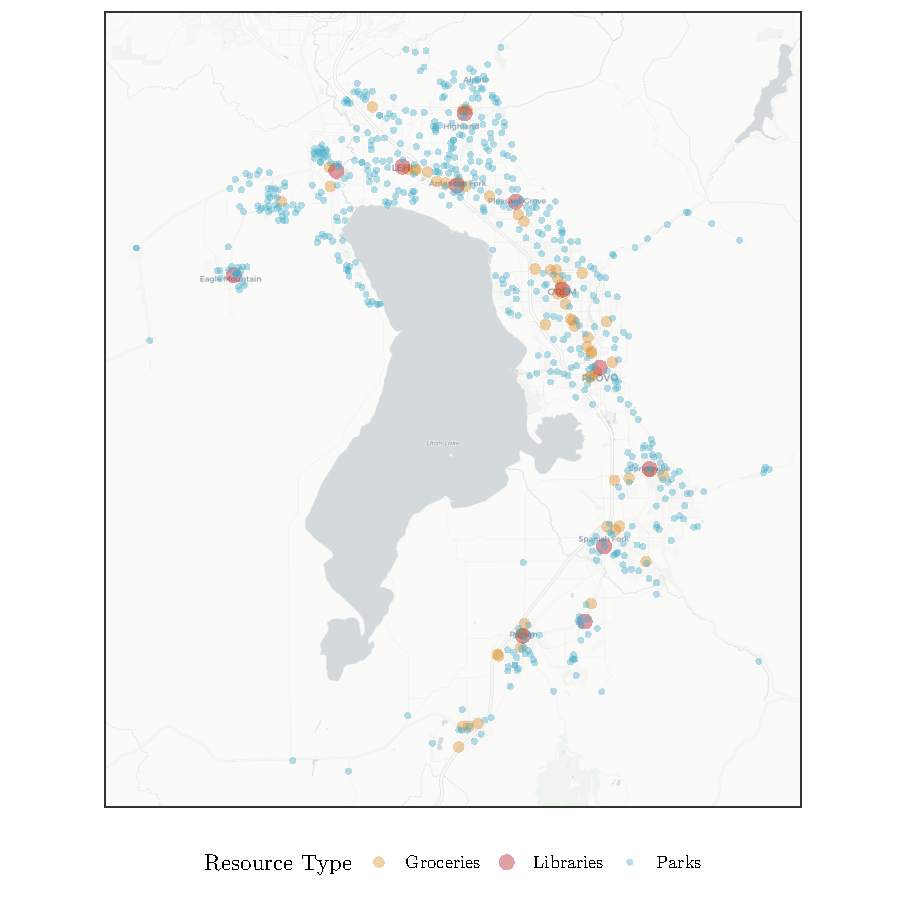
\includegraphics{Community_Resources_files/figure-latex/utco-map-1} 

}

\caption{Community Resources in Utah County}\label{fig:utco-map}
\end{figure}

\hypertarget{models}{%
\subsection{Models}\label{models}}

\hypertarget{results}{%
\section{Results}\label{results}}

\hypertarget{destination-choice-models}{%
\subsection{Destination Choice Models}\label{destination-choice-models}}

Using the simulated trip choices assembled from the location-based services data,
we estimate destination choice models with the \texttt{mlogit} package for
R \citep{R, mlogit}.

\begin{landscape}\begin{table}

\caption{\label{tab:park-models}Park Destination Choice Utilities}
\centering
\begin{tabular}[t]{lccccc}
\toprule
  & Car & MCLS & Attributes & All - Car & All - Logsum\\
\midrule
Drive time & -0.215(-95.949)** &  &  & -0.211(-70.944)** & \\
Mode Choice Logsum &  & 7.678(95.958)** &  &  & 7.512(70.948)**\\
log(Acres) &  &  & 1.447(86.983)** & 1.448(53.482)** & 1.448(53.469)**\\
Playground &  &  & 4.693(34.722)** & 4.632(31.107)** & 4.633(31.099)**\\
Volleyball &  &  & -0.312(-8.157)** & -0.564(-9.576)** & -0.565(-9.580)**\\
Basketball &  &  & -0.591(-13.940)** & -0.386(-5.651)** & -0.387(-5.663)**\\
Tennis &  &  & -0.612(-14.673)** & -0.974(-16.165)** & -0.976(-16.182)**\\
\midrule
Num.Obs. & 8,984 & 8,984 & 8,984 & 8,984 & 8,984\\
Log Likelihood & -9,288.8 & -9,284.7 & -12,348.3 & -4,974.7 & -4,971.6\\
McFadden Rho-Sq & 0.569 & 0.569 & 0.427 & 0.769 & 0.769\\
\bottomrule
\multicolumn{6}{l}{\textsuperscript{} t-statistics in parentheses. * p $<$ 0.5, ** p $<$ 0.1}\\
\end{tabular}
\end{table}
\end{landscape}

Table \ref{tab:park-models} presents the model estimation results for
five different specifications of park destination choice. The ``Car'' model
includes only the network travel time by car as a predictor of park choice;
the ``MCLS'' model similarly contains only the mode choice logsum as an
impedance term. The signs on the coefficient indicate that people are more
likely to choose parks with lower car distance or higher multi-modal access, all
else equal. The ``Attributes'' model includes only information on the park attributes
including size and amenities. On balance, people appear attracted to larger parks
and parks with playgrounds, while somewhat deterred by various sports facilities.
The ``All'' models include both the relevant travel impedance term as well as
destination attributes.

For most block group-park pairs, the transit and walk travel disutilities
are sufficiently high that choosing these travel modes is unlikely. As a
result, the mode choice logsum is highly collinear with the car travel time.
Nevertheless, there are small differences differences between the models
with the different impedance terms. Using a non-nested likelihood statistic
test presented by HOROWITZ, we can reject the null hypothesis that the two
``All'' models have equivalent likelihood (\(p\)-value of 0.00645), and infer
that the mode choice logsum is a marginally better estimator of park choice than
the vehicle travel time alone.

\begin{landscape}\begin{table}

\caption{\label{tab:grocery-models}Grocery Destination Choice Utilities}
\centering
\begin{tabular}[t]{lcccccc}
\toprule
  & Car & MCLS & Attributes & Size & All - Car & All - Logsum\\
\midrule
Drive time & -0.206(-90.014)** &  &  &  & -0.217(-78.388)** & \\
Mode Choice Logsum &  & 7.340(90.019)** &  &  &  & 7.733(78.399)**\\
Convenience Store &  &  & -2.339(-11.310)** & -1.600(-7.684)** & -1.486(-6.765)** & -1.488(-6.773)**\\
Other non-standard &  &  & -1.894(-14.604)** & -1.255(-9.554)** & -1.055(-7.487)** & -1.056(-7.490)**\\
Has pharmacy &  &  & 0.616(19.421)** & 0.329(8.901)** & 0.249(5.488)** & 0.249(5.502)**\\
Ethnic market &  &  & -1.680(-16.846)** & -0.997(-9.750)** & -0.883(-8.072)** & -0.884(-8.078)**\\
Has other merchandise &  &  & 1.523(48.309)** & 0.769(19.144)** & 0.881(17.631)** & 0.882(17.660)**\\
Number of registers &  &  &  & 0.073(42.117)** & 0.083(36.312)** & 0.083(36.294)**\\
Number of self-checkout &  &  &  & 0.031(15.255)** & 0.027(10.049)** & 0.027(10.041)**\\
\midrule
Num.Obs. & 8,404 & 8,404 & 8,404 & 8,404 & 8,404 & 8,404\\
Log Likelihood & -11,861 & -11,861.8 & -16,898.4 & -15,806.6 & -8,802.4 & -8,802.2\\
McFadden Rho-Sq & 0.411 & 0.411 & 0.161 & 0.216 & 0.563 & 0.563\\
\bottomrule
\multicolumn{7}{l}{\textsuperscript{} t-statistics in parentheses. * p $<$ 0.5, ** p $<$ 0.1}\\
\end{tabular}
\end{table}
\end{landscape}

Table \ref{tab:grocery-models} presents the model estimation results for the grocery
store models. As with the parks models in Table \ref{tab:park-models}, the
most predictive model contains both a travel impedance term and attributes of
the destination grocery store. The number of registers suggests that people
prefer larger stores, all else equal; ethnic markets, convenience stores, and other
facilities are less preferred while stores with pharmacies and other merchandise
(clothes, home goods, etc.) attract visitors. The ratio of the drive time and
convenience store coefficients suggests that on average, people are willing to
drive 6.86 minutes to reach a store that is not a convenience store.
In terms of the travel impedance, there is not a sufficiently large gap in the
model likelihoods to reject that the mode choice logsum and the drive
time are equivalent predictors of grocery store choice.

\begin{landscape}\begin{table}

\caption{\label{tab:library-models}Library Destination Choice Utilities}
\centering
\begin{tabular}[t]{lccccc}
\toprule
  & Car & MCLS & Attributes & All - Car & All - Logsum\\
\midrule
Drive time & -0.233(-95.379)** &  &  & -0.232(-89.281)** & \\
Mode Choice Logsum &  & 8.306(95.361)** &  &  & 8.270(89.266)**\\
Offers Classes &  &  & 1.318(44.405)** & 1.258(23.053)** & 1.257(23.033)**\\
Genealogy Resources &  &  & -1.127(-44.021)** & -1.024(-25.610)** & -1.024(-25.601)**\\
\midrule
Num.Obs. & 9,816 & 9,816 & 9,816 & 9,816 & 9,816\\
Log Likelihood & -10,841.9 & -10,840.3 & -21,944.4 & -10,322.5 & -10,321.7\\
McFadden Rho-Sq & 0.539 & 0.539 & 0.068 & 0.561 & 0.561\\
\bottomrule
\multicolumn{6}{l}{\textsuperscript{} t-statistics in parentheses. * p $<$ 0.5, ** p $<$ 0.1}\\
\end{tabular}
\end{table}
\end{landscape}

Table \ref{tab:library-models} presents the model estimation results for the
library destination choice models. As with parks and grocery stores, both
travel impedance and destination attributes are significant predictors of
library choice. In this case, however, the library attributes provide very little
predictive power of library choice. This is perhaps because virtually all
libraries in the dataset offer the same set of basic amenities, but also because
each municipality in Utah County tends to operate its own library rather than
having a system of interconnected library branches as might be typical in
larger cities or other regions. Additionally, there is no significant difference
between the prediction power of the mode choice logsum versus the car travel
time.

\hypertarget{accessibilities}{%
\subsection{Accessibilities}\label{accessibilities}}

\begin{figure}
\centering
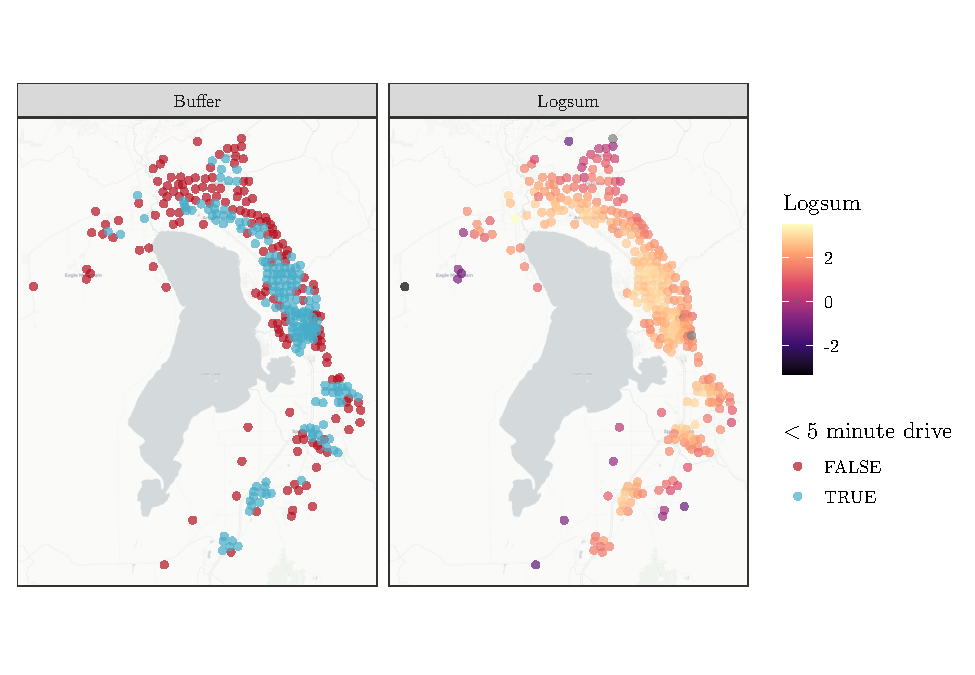
\includegraphics{Community_Resources_files/figure-latex/access-map-1.pdf}
\caption{\label{fig:access-map}Spatial comparison of grocery access buffer versus logsum.}
\end{figure}

\begin{figure}
\centering
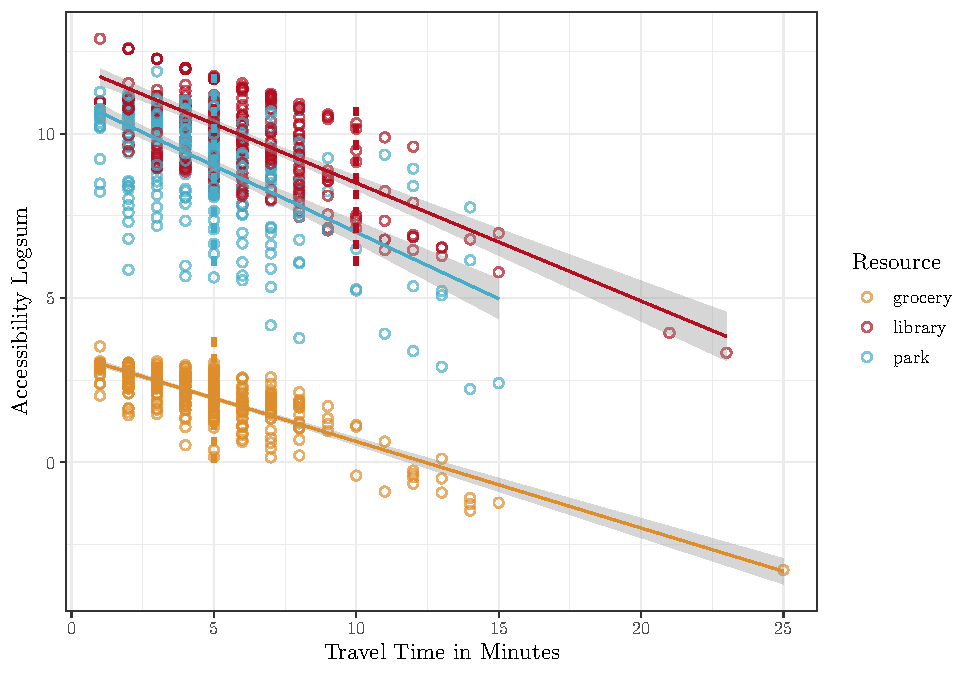
\includegraphics{Community_Resources_files/figure-latex/access-plot-1.pdf}
\caption{\label{fig:access-plot}Relationship between travel time, travel-time based buffer, and logsum value.}
\end{figure}

\hypertarget{limitations}{%
\section{Limitations}\label{limitations}}

The location-based services data reveals the likely home location of devices
observed within a geographic polygon, within some measurement error.
It cannot tell us whether the device holder actually accomplished the assumed
activity; that is, there may be a reason why a device was observed near a
library even though the person did not actually patronize the library.
Additionally, the method we use to compile the estimation dataset presumes that
the choice to make a trip to the community resource has already been made. Though
it can suggest how the accessibility of a neighborhood to these resource would improve
were transportation impedance decreased or the resources expanded or improved,
it cannot tell us how many more people might take advantage of the resource
in that case.

\hypertarget{acknowledgements}{%
\section*{Acknowledgements}\label{acknowledgements}}
\addcontentsline{toc}{section}{Acknowledgements}

The authors are grateful to Alisha Redelfs, Lori Spruance, Kaeli Monahan, and
Mali Smith for their help in gathering the grocery store information data.
Connor Williams gathered the parks data. Tables and figures in the article are
produced using a variety of packages for R \citep{modelsummary, ggspatial}

\bibliography{book.bib}


\end{document}
